\documentclass[dvipdfmx]{jsarticle}


\usepackage{tcolorbox}
\usepackage{color}
\usepackage{listings, plistings}

%% ノート/latexメモ
%% http://pepper.is.sci.toho-u.ac.jp/pepper/index.php?%A5%CE%A1%BC%A5%C8%2Flatex%A5%E1%A5%E2

% Java
\lstset{% 
  frame=single,
  backgroundcolor={\color[gray]{.9}},
  stringstyle={\ttfamily \color[rgb]{0,0,1}},
  commentstyle={\itshape \color[cmyk]{1,0,1,0}},
  identifierstyle={\ttfamily}, 
  keywordstyle={\ttfamily \color[cmyk]{0,1,0,0}},
  basicstyle={\ttfamily},
  breaklines=true,
  xleftmargin=0zw,
  xrightmargin=0zw,
  framerule=.2pt,
  columns=[l]{fullflexible},
  numbers=left,
  stepnumber=1,
  numberstyle={\scriptsize},
  numbersep=1em,
  language={Java},
  lineskip=-0.5zw,
  morecomment={[s][{\color[cmyk]{1,0,0,0}}]{/**}{*/}},
  keepspaces=true,         % 空白の連続をそのままで
  showstringspaces=false,  % 空白字をOFF
}
%\usepackage[dvipdfmx]{graphicx}
\usepackage{url}
\usepackage[dvipdfmx]{hyperref}
\usepackage{amsmath, amssymb}
\usepackage{itembkbx}
\usepackage{eclbkbox}	% required for `\breakbox' (yatex added)
\usepackage{enumerate}
\fboxrule=0.5pt
\parindent=1em
\begin{document}

%\anaumeと入力すると穴埋め解答欄が作れるようにしてる。\anaumesmallで小さめの穴埋めになる。
\newcounter{mycounter} % カウンターを作る
\setcounter{mycounter}{0} % カウンターを初期化
\newcommand{\anaume}[1][]{\refstepcounter{mycounter}{#1}{\boxed{\phantom{aa}\themycounter \phantom{aa}}}} %穴埋め問題の空欄作ってる。
\newcommand{\anaumesmall}[1][]{\refstepcounter{mycounter}{#1}{\boxed{\tiny{\phantom{a}\themycounter \phantom{a}}}}}%小さい版作ってる。色々改造できる。

%% 修正時刻: Tue May  5 10:19:29 2020


\section{PHPとJavaScript}

\subsection{PHPのはたらき}

PHPは、ユーザーがブラウザを通じて入力したデータを扱うことができる。
また、データベースに接続して、そこから取得したデータを扱うことができる。
PHPは、Webサーバーと連携して動作し、データをHTMLの中に埋め込むことができる。

だから PHPは、サーバーで動く。データを加工し、HTMLに埋め込む。
サーバーからクライアント(ブラウザ)に応答するときには、PHPはもう姿を消している。

\subsection{JavaScriptのはたらき}

では、JavaScriptはどうであろうか?

ためしに、以下のような HTML を書いてみる。そこに JavaScript を埋め込んでみる。

\begin{lstlisting}[caption=sample.html]
 <!doctype html>
 <html lang="ja">
   <head>
     <meta charset="utf-8">
     <title>sample</title>
   </head>
   <body>
     <h1>Sample</h1>
     <button id="button">ボタン</button>
     <script>
       const btn = document.getElementById('button')
       btn.onclick = function () {
         alert('Hello!')
       }
     </script>
   </body>
 </html>
\end{lstlisting}

上のコードを ``test''フォルダに ``sample.html'' という名前で保存する。

そして、``test'' フォルダで Webサーバーを起動する。(起動しっぱなしになっていてもよい)

Webサーバーの起動は、
\newsavebox{\samplebox}
\setbox\samplebox=\vbox{\hsize 5cm
\verb!> php -S localhost:8888!
}
\fbox{\usebox{\samplebox}}
で起動できる。

ブラウザで ``http://localhost:8888/sample.html'' にアクセスする。

\vspace{3mm}
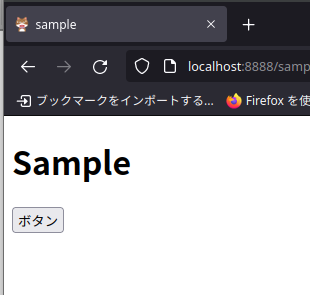
\includegraphics[width=8cm]{../img/51-sample.png}
\vspace{3mm}

このボタンをクリックすると、

\vspace{3mm}
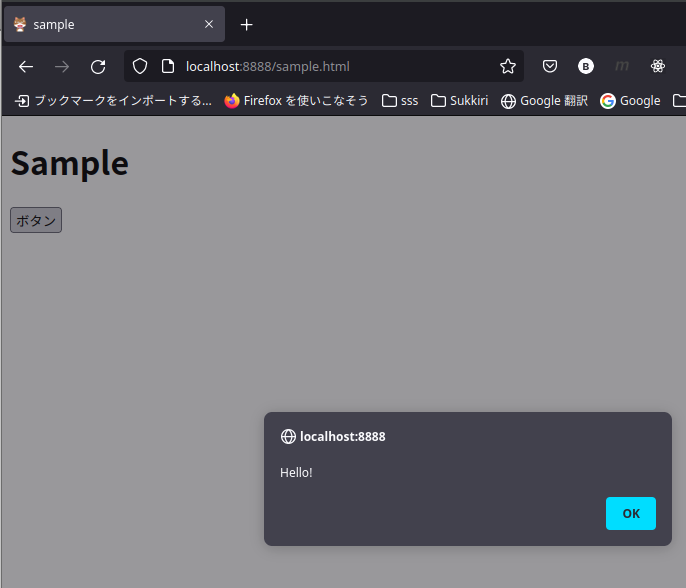
\includegraphics[width=13cm]{../img/52-sample-click.png}
\vspace{3mm}

と表示される。


\subsection{TeraTermでやってみる}

TeraTermで GET してみたら、どうだろうか?

Webサーバーが動作しているのを確認したのち、
TeraTermを起動する。

\begin{tabular}{lcl}
 ホスト & : & localhost \\
 サービス & : & Telnet \\
 TCPポート & : & 8888 \\
\end{tabular}

開いた黒い画面に以下を入力する。

\begin{tcolorbox}
 GET /sample.html HTTP/1.1 \\
 Host: localhsot:8888 \\
 (空行)
\end{tcolorbox}

ここで $<$Enter$>$ とすると、以下のように出力される。

\vspace{3mm}
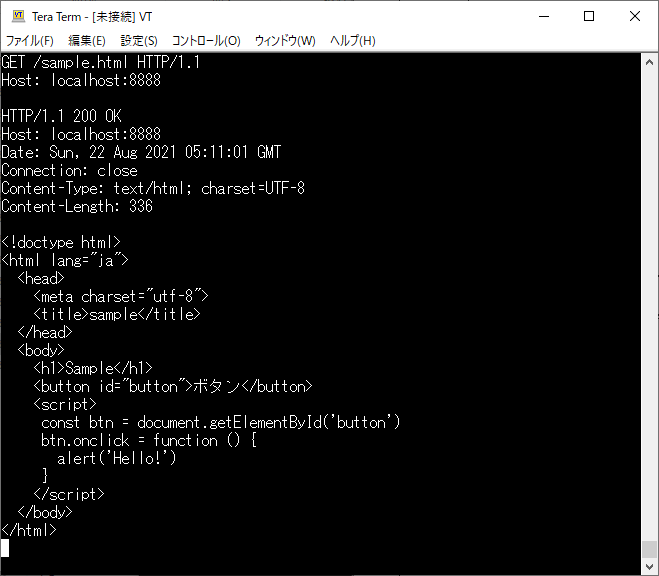
\includegraphics[width=13cm]{../img/53-sample-log.png}
\vspace{3mm}

\newsavebox{\samplelog}
\setbox\samplelog=\vbox{\hsize 12cm
\begin{verbatim}
HTTP/1.1 200 OK
Host: localhost:8888
Date: Sun, 22 Aug 2021 05:07:08 GMT
Connection: close
Content-Type: text/html; charset=UTF-8
Content-Length: 336

<!doctype html>
<html lang="ja">
  <head>
    <meta charset="utf-8">
    <title>sample</title>
  </head>
  <body>
    <h1>Sample</h1>
    <button id="button">ボタン</button>
    <script>
     const btn = document.getElementById('button')
     btn.onclick = function () {
       alert('Hello!')
     }
    </script>
  </body>
</html>
\end{verbatim}
}
\fbox{\usebox{\samplelog}}

このように JavaScript は HTML といっしょに Webサーバーから送られてくる。
そして、ユーザーのブラウザでレンダリングされ、そのときに JavaScript は
動作を始める。


\section{参考}

\href{https://atmarkit.itmedia.co.jp/ait/articles/0302/01/news001.html}{telnetでWebサーバに接続してみよう:TCP/IPアレルギー撲滅ドリル}


\end{document}

%% 修正時刻: Sat May  2 15:10:04 2020


%% 修正時刻: Wed Aug 25 06:19:11 2021
